\chapter{Bound Dirichlet Belief Model}\label{ccl}

\section{Introduction}
In this work, we propse Bound Dirichlet Belief Network to address the issue of DirBN model and enlarge the modelling capability. By inserting auxiliary Poisson random variables into the  layerwise connections and appropraite design.we assume that there are $N$ objects to be modelled in this word,where $\pi_{i'}$ is used to denote the $i'$-th latent distribution in the $l$-th layer.There are $L$ hidden layers in the deep architure.


\begin{figure}
% \centering % 图片居中
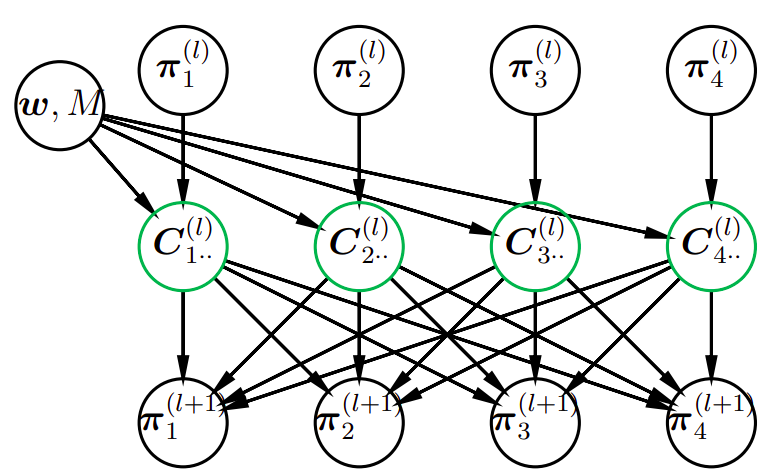
\includegraphics[width = \linewidth]{ubdn.png}
\caption{UBDN Model}
\label{fig:DirBN Model}
\end{figure}

$$ \pi_{i'.}^1 \sim Dirichlet(\beta) $$
$$C_{i'..}^{1} \sim Multi(M^l;\pi_{i'.}^1 \otimes w_{i'.}^l) \tag{1}$$
$$\pi_{i}^{2} \sim Dirihlet(\alpha_d +\sum_{i'}{C_{i'.i}})\tag{2}$$
$$\dots$$
$$C_{i'..}^{l} \sim Multi(M^l;\pi_{i'.}^l \otimes w_{i'.}^l) \tag{1}$$
$$\pi_{i}^{l+1} \sim Dirihlet(\alpha_d +\sum_{i'}{C_{i'.i}^l})\tag{2}$$
\begin{itemize}
  \item Information pass from Topic i' to Topic i;
  \item $\pi_{i'.}^l$ is the Topic-Word matrix in layer $l$;
  \item All layer has same Topic number;
  \item $w_{i'i}^l$ is the probability that information pass from topic i' to i;
  \item This is the reconstruction process;;
  \item  $\sum_{i'}{C_{i'.i}}$  is a (V*K) by 1 Vector;
\end{itemize}

where:
$$
M^{(l)} \sim Pisson(M)
$$
\[
w_{i'.}^l \sim Dirichlet(\eta)
\]
Since $\sum_k w_{i'k}^l =1$ ,we can further get :
$$
\sum_{i'}{C_{i'.i}} \sim Multinomial(M^{l};\pi_{i'}^l)
$$
That is to say, the normalized proportion vector can be ragard as an approximator of $\pi_{i'}^l$. We reorganiza the counting variables and calculate the recevied counts information for rach node $i$. For any node $i$, it will receive latent counts from all the nodes in this layer. These received counts can then be used to consistute the concentration parameter vector of the receiving node $i's$ Dirichlet distribution.

The number $M^{l}$ of events records the total intensity of relating the latent representation to the related counts. Larger
values of $M^{l}$ will remind a closer approximation to $\pi^{l}$. Further, the introduction of Poisson counts help to decompose the additive effect of the weights, which is quite difficult to have closed Gibbs sampling format.

This key contribution needs to be emphasized again. The
introduction of the counts variable $C$ enables us to use a
layerwise sampling method for all the variables and thus
avoid the complicated strategy of backward counts propagation and forward variable sampling. $C_{i'}^{{l}}$plays the role of “likelihood” variable for each latent distribution π and we can thus easily obtain Gibbs sampling for $\pi_{i'}^{(l)}$.
 Based on Poisson-Multinomial Equivalence,we can get:
 $$C_{i'ki}^{l} \sim Poisson(M^l \pi_{i'k}^l w_{i'i}^l)\tag{3}$$
 Combining its likelihood, we can easily obtain all its potential posterior proportional
 values.


\section{Inference Process}
Unlike DirBN model which inference latent vairiables by propagating count matrix with Chinese Restaurant Table (CRT) distribution.In DBN model,we can directly use Gibbs sampling stratrgy for model inference.
\begin{enumerate}
  \item Input matrix is topic-word matrix  $z$ which is a K by V matrix and then sample $\pi_{i'}^{L}$:

  $$\pi_{i'}^{L} \sim Dirichlet(z + C_{i'.i}^L)$$

  \item Sampling $C_{i'ki}^l$.
  $$P(C_{i'ki}^{l}|.) \sim \frac{(M^l \pi_{i'k}^l w_{i'i}^l)^{C_{i'ki}}}{C_{i'ki}^{l}!}$$

  $$P(\pi_i^{l+1}|C_{i'ki}^{l},..) = \frac{1}{B({\alpha_d +\sum_{i'}{C_{i'.i})}}} \prod^V \pi_{ik}^{\alpha_d+C_{i'ki}^l-1}$$

  The posterior distribution of $C_{i'ki}^{l}$ is:

  $$P(C_{i'ki}^{l}|.) \propto \frac{(M^l \pi_{i'k}^l w_{i'i}^l)^{C_{i'ki}}}{C_{i'ki}!} .\frac{1}{B({\alpha_d +\sum_{i'}{C_{i'.i}^{l})}}} \prod^V \pi_{ik}^{\alpha_d+C_{i'ki}^l-1} $$

  and

  $$\sum_{k,i}{C_{i'ki}^l} = M^l$$

  then

 $$
    {C_{i'ki}^l} \sim Mult(M^{l} | \frac{C_{i'..}^{l}}{\sum_{k,i} C_{i'ki}^{l}})
 $$


  \item Sampling $\pi_{i'}^l$,its posterior distribution is Dirichlet distribution.Given that :
  \[
    \pi_{i'..}^l \sim Dirihlet(\alpha_d +\sum_{i'}{C_{i'.i}^{(l-1)}})
  \]
  $$ \pi_{i'.}^1 \sim Dirichlet(\beta) $$
  \[
    \sum_i w_{i'i} = 1
  \]

  then :
    $$\sum_i{C_{i'ki}} \sim Multi(M^l;d\pi_{i'.}^l)$$
    $$
     \pi_{i'.}^l \sim Dirichlet(\eta + \sum_{i'} C_{i'.i}^{l-1} + \sum_i{C_{i'ki}^l})
    $$
    $$
     \pi_{i'.}^1 \sim Dirichlet(\beta +  \sum_i{C_{i'ki}})
    $$

  \item  Sampling $w_{i'}$.Given that:

  \[
    w_{i'}^l \sim Dirichlet(\eta)
  \]
  * Likelihood
  $$\sum_k{C_{i'ki}} \sim Multi(M^l;w_{i'.}^l)$$

  * Prior distribution

  $$W_{i'i} \sim Dirichlet(\alpha_w)$$

  * Posterior distribution

  $$p(w_{i'}|..) \sim Dirichlet(\alpha_w+w_{i'.})$$
\end{enumerate}

\section {Experiment}

The experiment was conduct on a real-word datsets called Tag My News (TMN) which contains 32597 RSS news labelled with 7 categories and there are 13370 unique words in the documents.

For UBD model,we set $M = 200,\eta = \beta = 1$

\begin{figure}[b]
% \centering % 图片居中
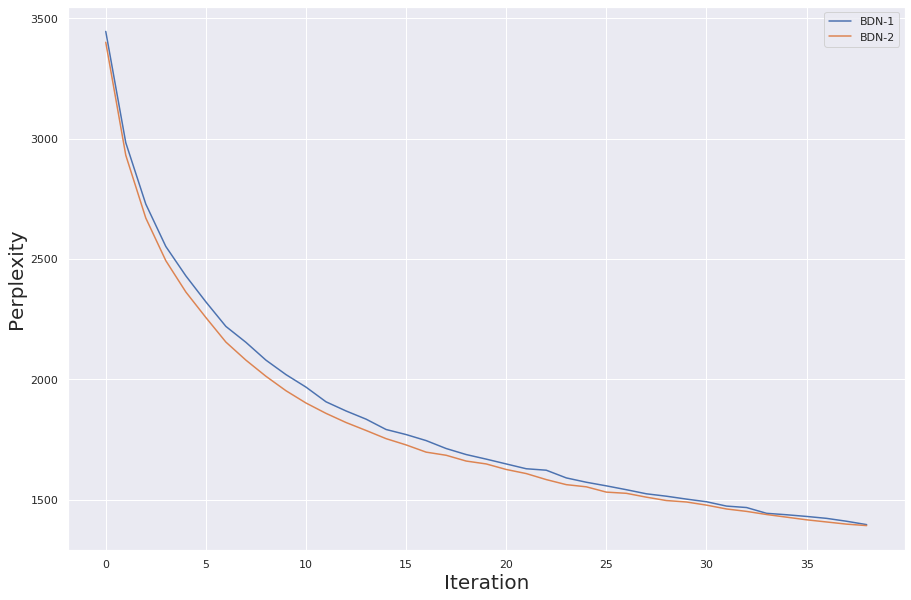
\includegraphics[width = \linewidth]{res.png}
\caption{Result of experiment}
\label{fig:DirBN Model}
\end{figure}


\chapter{Conclusion}\label{ccl}
We have present a new layerwise inference of Dirichlet Belief Model. With each topic in different layers, DBN model is able to deepen the uderstanding on topic hierarchies. By inserting auxiliary poisson random variable into the layerwise connections and appropriate design,direct efficient Gibbs sampling over random variables is available.

However,the limitation of this model is that the lengths of latent distrubutions in all the layers are restricted to be the same and need to be fixed.Further directions include introduction of Chinese Restaurant Process on the prior of the length of latent distribution
